\chapter{Extracellular conductivity}
\label{sec:Sigma}
\index{Conductivity}
\ghnote{GH: Planen var at dette skulle bli Torbjorns kapittel, men jeg laget en skisse.
Fint om Torbjorn sjekker alt jeg har foretatt meg, samt fyller ut med egne greier. Jeg sakset en del greier fra VC-kapittelet inn hit, blant annet delkapitlene om anisotropt og inhomogent medium. Pros: Naa utvider vi VC-teori i traad m/ at vi diskuterer (or relaxer) antakelser rundt sigma, jmf. tidligere versjon der vi utvidet VC teorien foerst, og deretter diskuterte og relaxet antakelsene. Cons: Naa blir det VC teori ogsaa i Sigma-kapittelet.}
\tvnnote{Egentlig syntes jeg mer kan flyttes hit, inkludert det med "Tortuous medium" og $\lambda$, og Figure 3.1? I så fall blir det i VC-teori bare en kort oppsumerring, omtrent slik som første avsnitt av "continuous, porus medium approximation for VC theory", samt en referanse til dette kapittelet. Jeg syntes hvertfall at alt bør være skrevet her også, slik at man ikke må lete etter informasjon om dette i forskjellige deler av boka.}

A key parameter, or sometimes, variable, in volume conductor (VC) theory is the extracellular conductivity, $\sigma_t$. In most applications of VC theory, $\sigma_t$ is assumed to be a constant, and its value is normally taken from some experimental measurement. Estimates can vary greatly between different recordings, but common values are between 0.2 and 0.3 S/m (Fig. \ref{Sigma:fig:freq_dep}). Throughout the previous section, we assumed that  $\sigma$  was homogeneous, anisotropic and frequency independent. In this chapter we shall discuss these assumptions. In addition, we discuss some experimental and theoretical estimates of  $\sigma_t$. Before doing so, however, we shall introduce the continuous, porous medium approximation in some detail, to show what $\sigma_t$ actually represents.


%%%%%%%%%%%%%%%%%%%%%%%%%%%%%%%%
\section{\blue{Continuous, porous medium approximation}}
\label{sec:Sigma:continuous}
\index{Continuous medium}
\index{Porous medium}

%%%%%%%%%%%%%%%%%%%%%%%%%%%%%%%%
When presenting the theory for modeling single neurons (Chapter \ref{sec:Neuron}), we may have given the impression that they are solitary creatures living in a vast extracellular space with long distances to their nearest cell neighbors. This is far from the truth. A cross-section of a piece of brain tissue shows that it is densely packed with neurons and glial cells (Fig.\ref{Sigma:fig:ECS}), and that the extracellular space (colored red in the figure) occupies only about 20 \% of the the total tissue volume. Moreover, it has a highly tortuous \index{Tortuosity} geometry, with an average intercell-distance of about 40-60 nm \cite{Sykova2008}. 

\begin{figure}[!ht]
\begin{center}
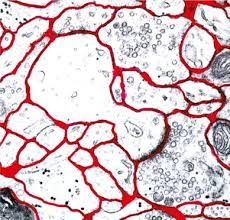
\includegraphics[width=0.3\textwidth]{Figures/Sigma/ECSdummy.jpeg}
\end{center}
\caption[]{\textbf{Tortuous medium}  Cross-section image of a piece of neural tissue. Extracellular space (marked red) occupies about 20 \% of the total tissue volume, and has a highly tortuous structure. Placeholder, taken from \cite{Sykova2008}.
\tvnnote{Vi får vel lage vår egen illustrasjon her, kanskje med panel A lik denne, og panel B en zoomet ut versjon der det ser mer homogent ut? Hadde Klas allerede laget en lignende figur til Sterratt? Dette bildet overdriver forresten situasjonen litt, siden det er fryse-tørket eller noe slikt, så mesteparten av CSFen er tatt bort.}
}
\label{Sigma:fig:ECS}
\end{figure}

At the microscopic scale, the conductivity \index{Conductivity} $\sigma$ in the brain tissue is thus highly non-homogeneous. For example, it will be very high at a cellular membrane and much lower in the extracellular space between membranes. Accordingly, electric potentials can vary greatly over tiny distances, and become very large near cell membranes. When we study extracellular potentials, we are typically not interested in these microscopic variations in $\sigma$ and $\phi$, but rather in the values of these entities when averaged over some spatial volume. In practice, the electrodes used in experimental recordings perform such an averaging. Sizes of electrodes used to record extracellular potentials typically range from 5 $\mu$m to 125 $\mu$m in diameter\cite{Viswam2019}, which is larger than the typical diameter of a dendrite ($\sim$ 1 $\mu$m). Experimental recordings thus give us the average potential over a region in space that typically spans over both extracellular space and several neural and glial processes. It is thus the dynamics at this coarse grained spatial scale that we will focus on.

At the coarse grained spatial scale, it is reasonable to assume that microscale inhomogeneities average out, and that the brain tissue can be treated as a continuous medium \cite{Gratiy2017}. The VC theory presented in the previous chapter was based on the continuous medium approximation, and thus describes the extracellular dynamics on a coarse grained spatial scale, with a spatial resolution larger than a micrometer. 

A continuous, porous medium is defined by two key parameters \cite{Nicholson1981}. The first parameter is $\alpha$, is the fraction of the tissue volume that is extracellular space. A typical value for $\alpha$ in brain tissue is 0.2, although this can vary between brain regions and even locally due to cellular swelling or shrinkage. The second parameter is $\lambda$, the tortuousity of the medium \cite{Nicholson1981}. It is defined as the ratio between the shortest pathway between two points in space and the euclidian distance between these two points, and accounts for the fact that ions traveling through the medium do not travel in straight lines, but need to take detours around cellular obstacles. The tortuosity can be measured experimentally, and for extracellular transport, it has been found that $\lambda = 1.6$ \cite{Nicholson1998}. 

The continuous, tortuous medium approximation has implications for how we interpret the various concepts and variables that we use. For example, in the previous Chapter we used the term "extracellular medium" \index{Extracellular medium}, to refer to brain tissue as it is \textit{experienced} by macroscopic extracellular currents. Importantly, the extracellular medium is not the same as the "extracellular solution" \index{Extracellular solution}, i.e. the fluid filling the extracellular space. Although extracellular currents indeed pass through the extracellular solution, they do not pass through a 3D volumed filled exclusively by this solution. Instead they pass through the extracellular medium, defined as a medium where they (i) are confined to move only through a fraction $\alpha$ of the total medium volume, and (ii) must take detours around neural and glial obstacles, as reflected through the tortuousity $\lambda$ \cite{Nicholson1998,Nunez2006}. 

The (macroscopic) extracellular conductivity $\sigma_t$ (S/m) \index{Conductivity} is thus not the same as the (microscopic) conductivity of the extracellular solution, but the coarse-grained conductivity of the extracellular medium as defined above, so that the reduced volume fraction and tortuousity are accounted for. Experimental recordings of the extracellular conductivity typically measure $\sigma_t$ as defined in this way. For comparison, the microscopic and unhindered conductivity of the (pure) extracellular solution $\sigma_{saline}$ should theoretically be a fraction $\lambda^2/\alpha$ higher. 


%%%%%%%%%%%%%%%%%%%%%%%%%%%%%%%%
\section{\blue{Anisotropic extracellular medium}}
\label{sec:Sigma:Anisotropic}
\index{Conductivity!Anisotropic}

%%%%%%%%%%%%%%%%%%%%%%%%%%%%%%%%
In Chapter \ref{sec:VC}, we assumed that the extracellular conductivity $\sigma_t$ was isotropic, i.e., the same in all spatial directions. It is relatively straightforward to expand the VC theory to the case of an anistotropic $\sigma_t$. If we use the point source approximation (eq. \ref{VC:eq:pointsources}), and denote the conductivity in the different spatial directions $\sigma_{tx}$, $\sigma_{ty}$ and $\sigma_{tz}$, the extracellular potential surrounding a set of point current sources $I_k$ is given by \cite{nicholson1975,Pettersen2012}:

\begin{equation}
\phi(x,y,z) = \sum_k \frac{I_k}{4\pi(\sigma_{ty}\sigma_{tz} (x-x_k)^2 + \sigma_{tx}\sigma_{tz} (y-y_k)^2 + \sigma_{tx}\sigma_{ty} (z-z_k)^2)}.
\label{Sigma:eq:Panisos}
\end{equation}
If we use the CSD-description of the sources (eq. \ref{VC:eq:csds}, the corresponding expression is:

\begin{equation}
\phi(x,y,z) = \iiint_V \frac{C(x,y,z)}{4\pi(\sigma_{ty}\sigma_{tz} (x-x_k)^2 + \sigma_{tx}\sigma_{tz} (y-y_k)^2 + \sigma_{tx}\sigma_{ty} (z-z_k)^2)} \, dV, 
\label{Sigma:eq:Canisos}
\end{equation}

In general, the brain does not have an isotropic $\sigma_t$. For example, in cortex it has been found that the conductivity is about 50\% higher in the depth direction, i.e., for currents running in parallel to the axis of pyramidal cell dendrites \cite{Goto2010}. However, the overall effect of the anisotropy on extracellular potentials often appears to be quite weak \cite{Ness2015,Miceli2017}, and the approximation that $\sigma_t$ is isotropic often gives good predictions of the potential.


%%%%%%%%%%%%%%%%%%%%%%%%%%%%%%%%
\section{\red{TVN: Nonhomogeneous extracellular medium}}
\label{sec:Sigma:nonhomo}
\index{Conductivity!Nonhomogeneous}

In Chapter \ref{sec:VC}, we assumed that the extracellular conductivity $\sigma_t$ was homogeneous, i.e., the same everywhere. Clearly, this assumption does not hold on the micrometer scale, where neural tissue is highly non-homogeneous \cite{Nicholson1998}. However, microscale inhomogeneities tend to average out on a larger spatial scale (cf. the continuous medium approximation), and a homogeneous conductivity appears to be a reasonable approximation, at least within a given brain region such as cortex \cite{Logothetis2007}. 

The situation is different when signals are recorded very far from their sources. It is then likely that they on their journey have experienced a $\sigma_t$ that varied on a macroscopic scale. For example, the signals recorded in the EEG have traveled through brain tissue, bone and skin, which are three different media with different conductivities. When $\sigma_t$ is non-homogeneos, there is no general analytical formula available (like eqs. \ref{VC:eq:csds} or \ref{VC:eq:anisos}) that link the extracellular potentials to the underlying current sources. However, analytical solutions can still be obtained for some simple and idealized non-homogeneous cases. 

\ghnote{Enter TVN:}
\begin{itemize}
\item Method of Images \cite{Ness2015}
\item FEM \cite{Ness2015}, ...
\end{itemize}

For more general cases, one can in principle always solve eq. \ref{VC:eq:CSD2} for arbitrarily complex geometries with varying conductivities using numerical methods, like the Finite Element Method (FEM) \cite{Logg2012}. For examples of neuroscience applications using this approach, see \cite{Moffitt2005,Frey2009,Joucla2012,Haufe2015,Ness2015,Buccino2019b,Obien2019}. 

%%%%%%%%%%%%%%%%%%%%%%%%%%%%%%%%

\section{\orange{TVN: Frequency dependence of the conductivity} }
\label{sec:Sigma:f-independent}
\index{Conductivity!Frequency dependence}
\ghnote{GH: Skrev skisse til dette. Puttet figuren m/ sigma-maalinger inn her, da disse ser ut til aa primaert diskuteres opp mot eventuell frekvensavhengighet. Mulig vi burde ha med "eksperimentelle maalinger i kapittel-tittelen?}

Regardless of whether a medium is isotropic and homogeneous or not, its response to an imposed alternating current can depend on the frequency of the current. Then, the conductivity contains a resistive part, which is real and frequency independent, and an imaginary part that account for capacitive and inductive effects that are frequency dependent. 

In Section \ref{sec:VC:onlyohmic}) we argued that the extracellular displacement current is negligible, which means that the extracellular medium in itself does not exhibit any capacitive effects. This alone does not rule out the possibility that the effective conductivity of the tissue medium includes capacitive effects, as an extracellular current traveling through it could interact with nearby capacitive neural membranes. 

However, for the relevant frequencies in extracellular recordings (Fig. \ref{Sigma:fig:freq_dep}), the capacitive and inductive effects appear to be negligible compared to the resistive effects \cite{Logothetis2007,Miceli2017,Ranta2017}. In most applications of VC theory, one therefore applies the assumption that the medium is Ohmic or resistive, meaning that the imaginary and frequency dependent part of the conductivity is zero. We note, however, that it is possible to expand the formalism to include a frequency dependent conductivity \cite{Bedard2004,Tracey2011,Miceli2017}. 

\begin{figure}[!ht]
\begin{center}
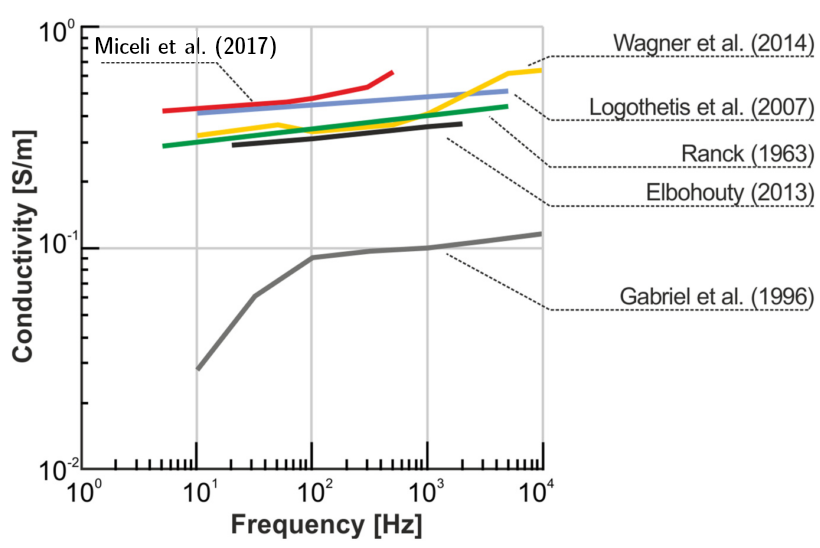
\includegraphics[width=0.6\textwidth]{Figures/Sigma/frequency_dependence.png}
\end{center}
\caption[]{\textbf{Literature review of reported conductivities in various species and experimental setups.} 
Most studies seem to indicate a very weak frequency dependence of the extracellular conductivity\index{Conductivity}, which would have a negligible effect on measured extracellular potentials \cite{Miceli2017}. The very low and strongly frequency dependent values measured by \cite{Gabriel1996} represents an outlier, and although it has received substantial attention, it has to the best of our knowledge not been reproduced by any other study. For details about the data, see \cite{Miceli2017}, and references therein \cite{Ranck1963,Gabriel1996,Logothetis2007,Elbohouty2013,Wagner2014}.
}
\label{Sigma:fig:freq_dep}
\end{figure}

\tvnnote{Utledning tilsvarende Appendix B i Nunez?}
\ghnote{Vet ikke helt.... Kanskje.... }


\begin{figure}[!ht]
\begin{center}
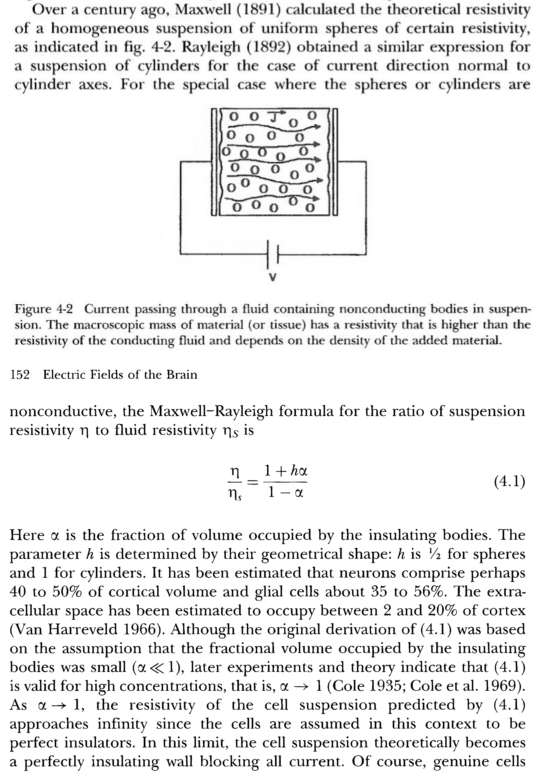
\includegraphics[width=0.6\textwidth]{Figures/Sigma/resistivity_maxwell.png}
\end{center}
\caption{\textbf{From Nunez} \tvnnote{Ta med noe slikt?}}
\label{Sigma:fig:maxwell_resistivity}
\end{figure}

\section{\red{TVN: Theoretical explorations....} }
\index{Conductivity!Theoretical estimates}

\ghnote{Dette var et punkt i den opprinnelige planen. Referenser: Meffin2012, 
Tahayori2012, Meffin2014, Tahayori2014. Jeg vet ikke helt hva dette gaar i, men det gjoer sikkert Torbjorn og/eller Gaute?}


\section{\blue{GH: Theoretical estimate of the conductivity based on ion concentrations} }
\label{sec:Sigma:concentrationbased}
\index{Conductivity!Ion concentration dependence}

Extracellular current are mediated by the ions dissolved in the extracellular solution, and the conductivity of the extracellular medium if thus a function of thus depends on the ion concentrations, i.e., on the availability of free charge carriers \cite{Grodzinsky2011}: 

\begin{equation}
\sigma_{saline} = \frac{F^2}{RT}\sum_{k} D_k z_{k}^2 c_{k}.
\label{Sigma:eq:sigma1}
\end{equation}
Here $z_{k}$, $D_k$ and $c_{k}$ denote the valency, diffusion coefficient and concentration, respectively, of ion species $k$, while $F = 96485.3$ C/mol is the Faraday constant, $R = 8.314$ JK$^{-1}$mol$^{-1}$ is the gas constant, and $T$ the temperature. 

Eq. \ref{Sigma:eq:sigma1} allows us to compare the measured $\sigma_t$ with $\sigma_{saline}$ as predicted from the typical ion concentrations in the extracellular space of the brain, such as those listed previously in Table \ref{table:ion-concentrations}. For this, we also need the diffusion constants of these species. In a dilute solution, such as the extracellular fluid, these are as given in Table \ref{Sigma:tab:diffconsts}.

\begin{table}[h!]
\begin{center}
\caption[Diffusion Constants]{Diffusion constants. Values taken from from \cite{Bowen2002,Lyshevski2007}}
\label{Sigma:tab:diffconsts}
    \begin{tabular}{l|l}
    \hline
    $D_{Na}$ & $1.33\times 10^{-9}$ m$^2$/s\\ \hline
    $D_K$ & $1.96  \times 10^{-9}$ m$^2$/s \\ \hline
    $D_{Cl}$ & $2.03 \times 10^{-9}$ m$^2$/s \\ \hline
    $D_{Ca}$ & $0.71\times 10^{-9}$ m$^2$/s \\ \hline
    $D_{Mg}$ & $0.72\times 10^{-9}$ m$^2$/s \\ \hline    
    $D_{HCO3}$ & $1.18\times 10^{-9}$ m$^2$/s \\ \hline
    \end{tabular}
\end{center}
\end{table}

If we insert the values from Tables \ref{Neuron:tab:ion-concentrations} and \ref{Sigma:tab:diffconsts} into equation \ref{Sigma:eq:sigma1}, and assume a body temperature of $T = 310$ K, we get a conductivity $\sigma_{saline} = 1.72$ S/m. This is a factor 6-9 times higher than the values (0.2-0.3 S/m) which are typically measured for the tissue conductivity. 

Currents through brain tissue do not move through a pure ion solution, and the effective tissue conductivity $\sigma_t$ is lower than $\sigma_{saline}$ for two main reasons. Firstly, extracellular currents are confined to stay in the small fraction $\alpha$ of the tissue volume that is extracellular, so that only a fraction $\alpha$ of the tissue volume has the conductivity predicted by eq. \ref{Sigma:eq:sigma1}. Secondly, even within the extracellular volume fraction, eq. \ref{Sigma:eq:sigma1} overestimates the conductivity, because extracellular currents will encounter obstacles (neural and glial membranes) along their path, forcing them take detours that can be quantified through a tortuosity factor $\lambda$. 

If we correct eq. \ref{Sigma:eq:sigma1} for the extracellular volume fraction and tortuous structure of the extracellular space, we get an estimate for the effective tissue conductivity as \cite{Okada1994}:
\begin{equation}
\sigma_{t} = \frac{\alpha}{\lambda^2} \sigma_{saline}.
\label{Sigma:eq:sigmat}
\end{equation}
Typical values for $\alpha$ and $\lambda$ for the extracellular space of brain tissue are 0.2 and 1.6, respectively \cite{Nicholson1981,Nicholson1998}. With these values, $\sigma_t$ becomes almost a factor 13 lower than $\sigma_{saline}$. 

With our above estimate of $\sigma_{saline}$, we get a an estimated tissue conductivity $\sigma_t = 0.134$ S/m. This is lower than the typical measured values for $\sigma_t$, which, although they vary quite much between different experiments, tend to be $> 0.2$ S/m. The main explanation to why our $\sigma_t$ is an underestimate is probably that it is based on the assumption that all tissue currents are confined to the extracellular space, while a fraction of the real tissue currents may also travel through the intracellular medium. For example, in cerebellum, it has been estimated that about 50 \% of tissue currents travel through intracellular paths \cite{Okada1994}. An additional explanation is that the extracellular solution contains many ions (such as e.g., H$^+$ and HPO4$^{2-}$ ) that we did not include in Table \ref{Neuron:tab:ion-concentrations} and thus not in our calculation of $\sigma_t$. However, since concentrations of ions others than those in Table \ref{Neuron:tab:ion-concentrations} are quite low, they will probably have only a minor impact on the conductivity. 

As we shall see in Chapter \ref{sec:Eldiff}, the definition of $\sigma_t$ given by eq. \ref{Sigma:eq:sigmat} follows naturally if we use the Nernst-Planck equation for electrodiffusive ion concentration dynamics to compute extracellular currents. 
